% MIT License
% 
% Copyright (c) 2022 cgsdfc
% 
% Permission is hereby granted, free of charge, to any person obtaining a copy
% of this software and associated documentation files (the "Software"), to deal
% in the Software without restriction, including without limitation the rights
% to use, copy, modify, merge, publish, distribute, sublicense, and/or sell
% copies of the Software, and to permit persons to whom the Software is
% furnished to do so, subject to the following conditions:
% 
% The above copyright notice and this permission notice shall be included in all
% copies or substantial portions of the Software.
% 
% THE SOFTWARE IS PROVIDED "AS IS", WITHOUT WARRANTY OF ANY KIND, EXPRESS OR
% IMPLIED, INCLUDING BUT NOT LIMITED TO THE WARRANTIES OF MERCHANTABILITY,
% FITNESS FOR A PARTICULAR PURPOSE AND NONINFRINGEMENT. IN NO EVENT SHALL THE
% AUTHORS OR COPYRIGHT HOLDERS BE LIABLE FOR ANY CLAIM, DAMAGES OR OTHER
% LIABILITY, WHETHER IN AN ACTION OF CONTRACT, TORT OR OTHERWISE, ARISING FROM,
% OUT OF OR IN CONNECTION WITH THE SOFTWARE OR THE USE OR OTHER DEALINGS IN THE
% SOFTWARE.

\begin{figure}[htb]
    \begin{subfigure}{0.35\linewidth}
        \centering
        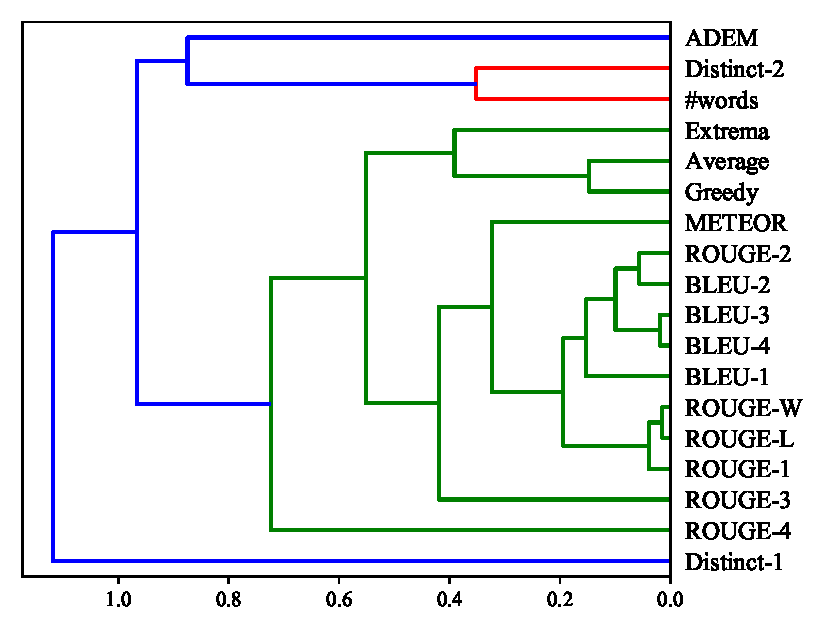
\includegraphics[width=\linewidth]{figure/plot/hierarchy/v3/pearson/hred/lsdscc/plot.pdf}
        \caption{(HRED, LSDSCC)}
    \end{subfigure}%
    \begin{subfigure}{0.35\linewidth}
        \centering
        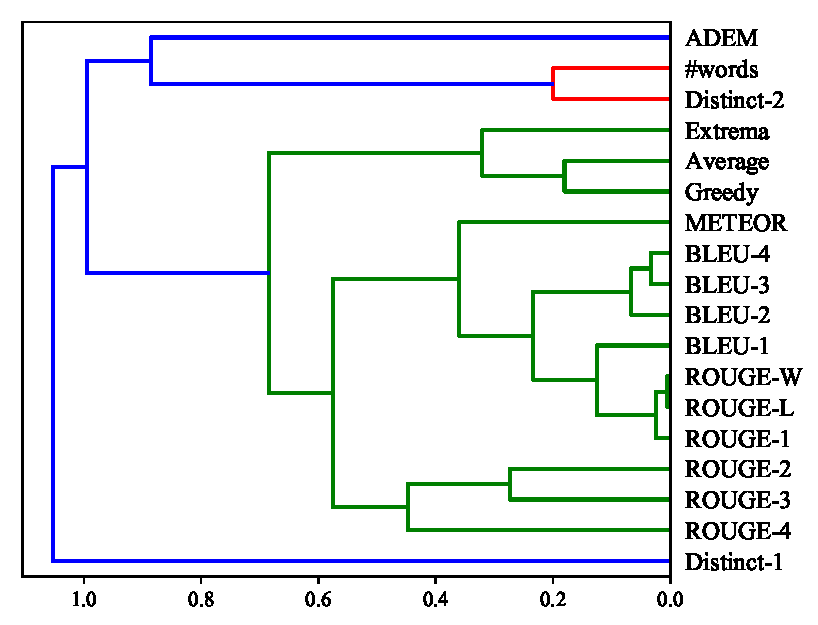
\includegraphics[width=\linewidth]{figure/plot/hierarchy/v3/pearson/hred/opensub/plot.pdf}
        \caption{(HRED, OpenSubtitles)}
    \end{subfigure}%
    \begin{subfigure}{0.35\linewidth}
        \centering
        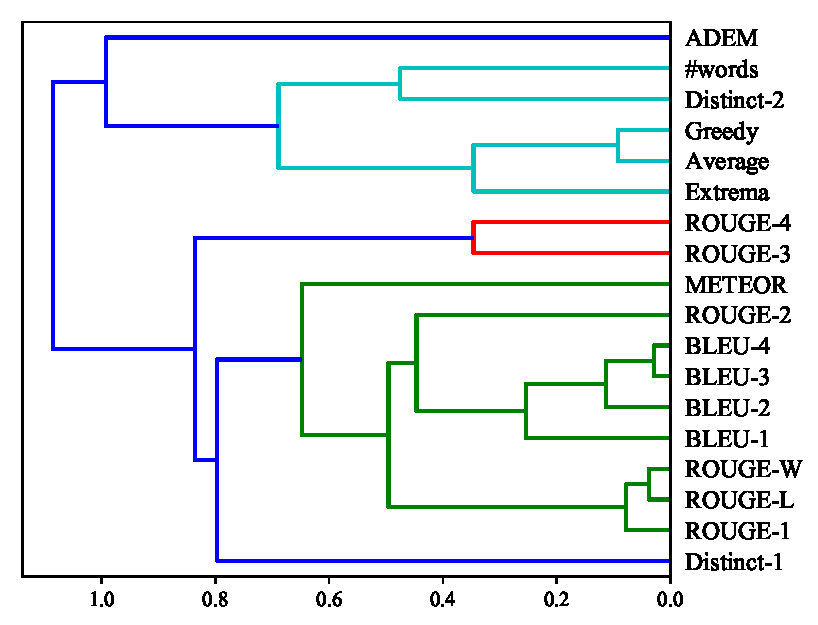
\includegraphics[width=\linewidth]{figure/plot/hierarchy/v3/pearson/hred/ubuntu/plot.pdf}
        \caption{(HRED, Ubuntu)}
    \end{subfigure}
    \begin{subfigure}{0.35\linewidth}
        \centering
        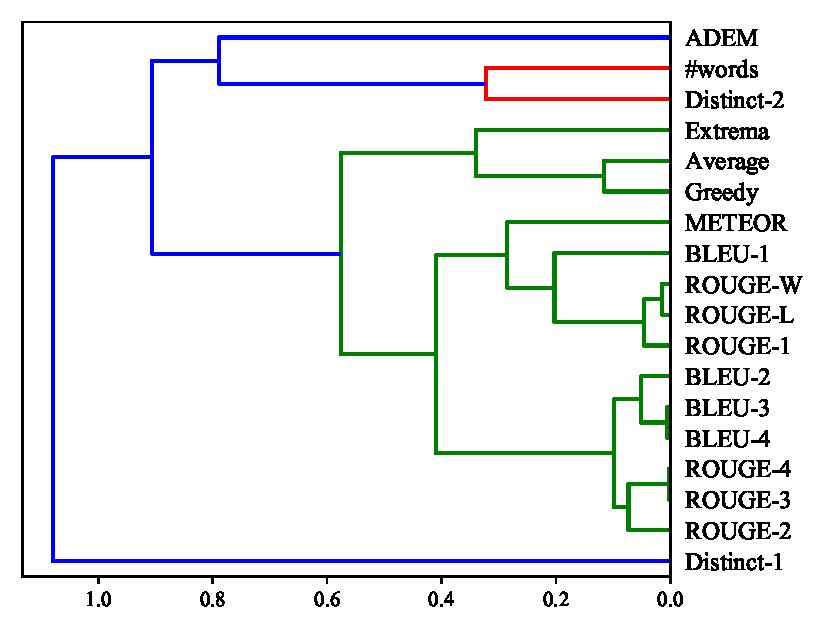
\includegraphics[width=\linewidth]{figure/plot/hierarchy/v3/pearson/vhred/lsdscc/plot.pdf}
        \caption{(VHRED, LSDSCC)}
    \end{subfigure}%
    \begin{subfigure}{0.35\linewidth}
        \centering
        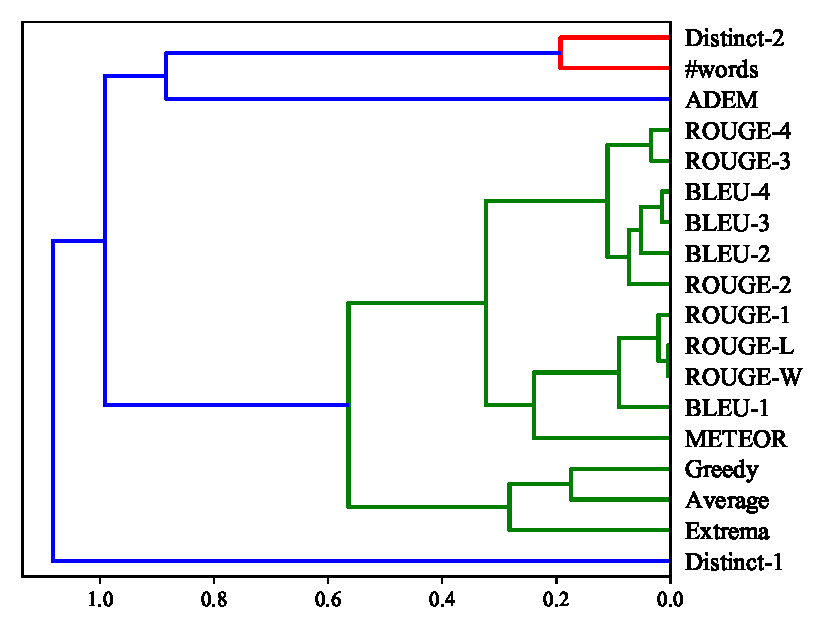
\includegraphics[width=\linewidth]{figure/plot/hierarchy/v3/pearson/vhred/opensub/plot.pdf}
        \caption{(VHRED, OpenSubtitles)}
    \end{subfigure}%
    \begin{subfigure}{0.35\linewidth}
        \centering
        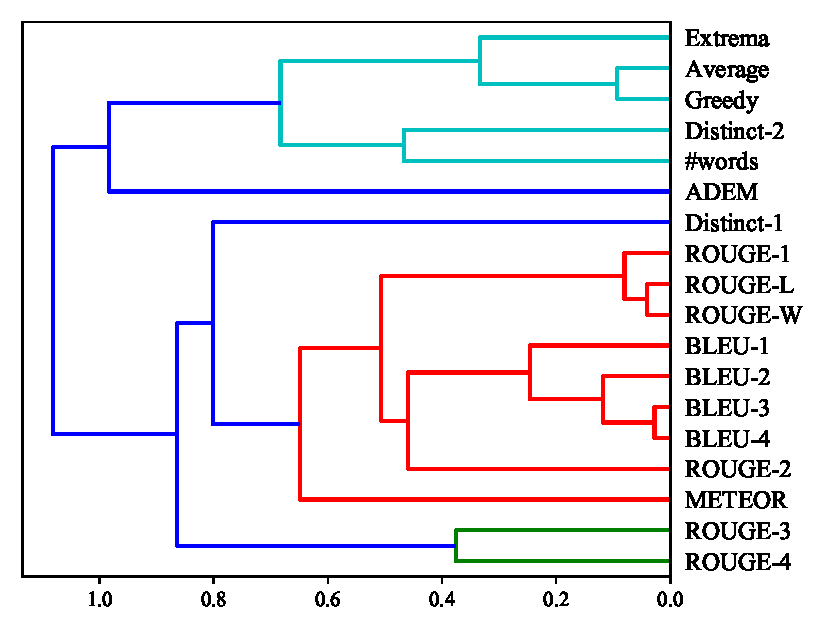
\includegraphics[width=\linewidth]{figure/plot/hierarchy/v3/pearson/vhred/ubuntu/plot.pdf}
        \caption{(VHRED, Ubuntu)}
    \end{subfigure}
    \begin{subfigure}{0.35\linewidth}
        \centering
        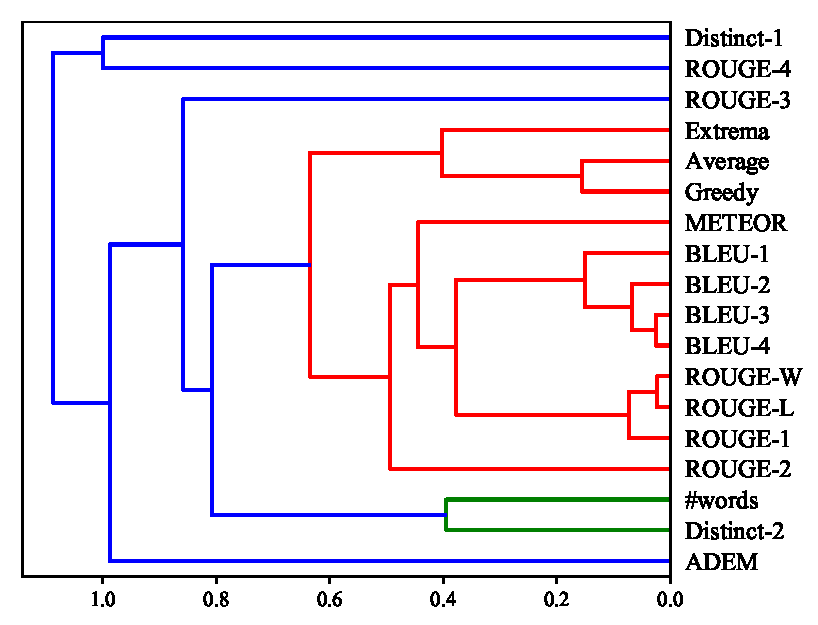
\includegraphics[width=\linewidth]{figure/plot/hierarchy/v3/pearson/lstm/lsdscc/plot.pdf}
        \caption{(LSTM, LSDSCC)}
    \end{subfigure}%
    \begin{subfigure}{0.35\linewidth}
        \centering
        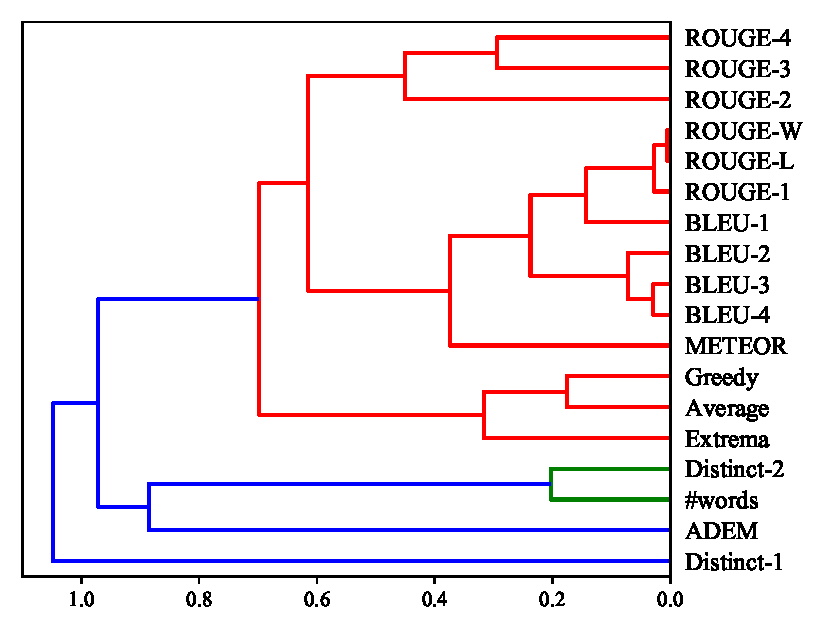
\includegraphics[width=\linewidth]{figure/plot/hierarchy/v3/pearson/lstm/opensub/plot.pdf}
        \caption{(LSTM, OpenSubtitles)}
    \end{subfigure}%
    \begin{subfigure}{0.35\linewidth}
        \centering
        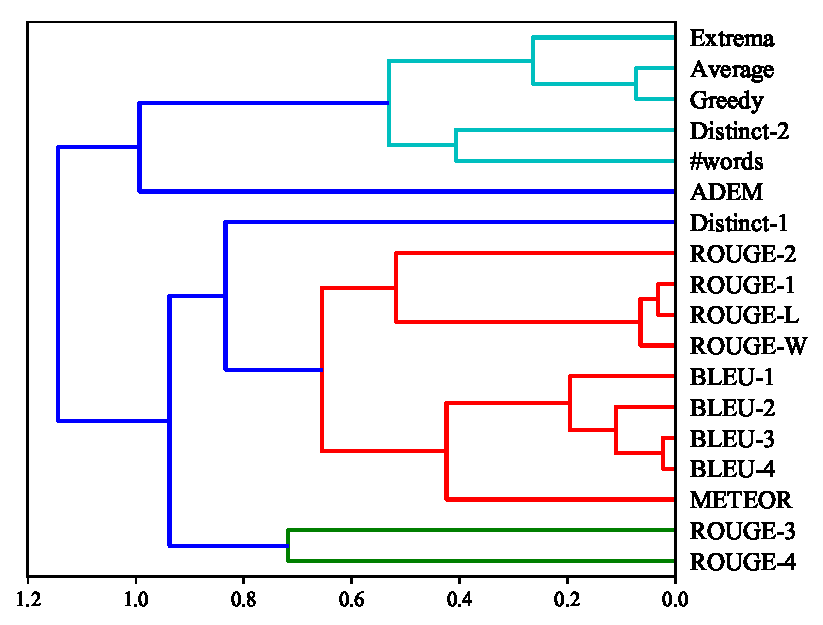
\includegraphics[width=\linewidth]{figure/plot/hierarchy/v3/pearson/lstm/ubuntu/plot.pdf}
        \caption{(LSTM, Ubuntu)}
    \end{subfigure}
    \centering
    \caption{Hierarchical Clusterings with Pearson's r}
    \label{fig:hierarchy}
\end{figure}
